\section{Lexikalische Konventionen, Enum \verweis{4}}
 	\subsection{Bestandteile des Sourcecodes}
 		\begin{minipage}[t]{5.5 cm}
 			\subsubsection{Lexikalische Elemente ("'Text"')}
 				\begin{compactitem}
 					\item Befehle
 					\item Variablen
 					\item Deklarationen
 					\item ... 
 				\end{compactitem}
 		\end{minipage}
 		\hspace*{3.5cm}
 		\begin{minipage}[t]{8 cm}
 			\subsubsection{Trennzeichen}
 				\begin{compactitem}
 					\item Leerzeichen
 					\item Tabulatoren
 					\item Newline
 				\end{compactitem}
 		\end{minipage}
 		
%%%%%%%%%%%%%%%%%%%%%%%%%%%%%%%%%%%%%%%%%%%%%%%%%%%%%%%%%%%%%%%%%%%%%%%%%%%%%%%%%%%%%%%%%%%%%%%%%%%%%%%%%	
\newpage%%%%%%%%%%%%%%%%%%%%%%%%%%%%%%%%%%%%%%%%%%%%%%%%%%%%%%%%%%%%%%%%%%%%%%%%%%%%%%%%%%%%%%%%%%%%%%%%%
%%%%%%%%%%%%%%%%%%%%%%%%%%%%%%%%%%%%%%%%%%%%%%%%%%%%%%%%%%%%%%%%%%%%%%%%%%%%%%%%%%%%%%%%%%%%%%%%%%%%%%%%% 	
	
 	\subsection{Zeichenvorrat von C \verweis{4.1}}
 		Der Zeichenvorrat für einen Quelltext in C umfasst: \\
 		\begin{minipage}[c]{9 cm}
 			\begin{compactitem}
 				\item Grosse und kleine Buchstaben, keine Umlaute: A - Z, a - z 
 				\item Unterstrich: \_
 				\item Ziffern: 0 - 9
 				\item Leerzeichen (Blank, Space), Tabulator
 				\item Strichpunkt (Semikolon): ;	
 			\end{compactitem}  				
 		\end{minipage}
 		\hspace*{0.5cm}
 		\begin{minipage}[c]{9 cm}
			\begin{compactitem}
 				\item Punkt (Dezimaltrennung, Selektionsoperator): .
 				\item Sonderzeichen für Operatoren: ( ) \ \ [ ] \ \ \textless  	\textgreater \ \  + \ \ - \ \ * \ \ / \ \ \% \ \ \^ \ \ \textasciitilde \ \ \& \ \ | \ \ = \ \ ! \ \ ? \ \ :
 				\item Hochkomma, Doppelhochkomma: ' \ \ "'
 				\item Geschweifte Klammern: \{ \}
 				\item (Hash), Sharp, "'Gartenhag"': \#
 				\item Backslash: \textbackslash 	
 			\end{compactitem} 
 		\end{minipage}

 	\subsection{Lexikalische Analyse des Sourcecodes}
 		\begin{minipage}[c]{10 cm}
 			\subsubsection{Scanner}
 				Zeichengruppen finden. Alle zusammengehörenden
 				Zeichengruppen, welche nicht durch einen Trenner 
 				(z.B. Operator oder Trennzeichen) unterbrochen werden, gelten als lexikalische Einheiten (Token).
 			\vspace*{0.5cm}
 		 	\subsubsection{Parser}
 		 		lexikalische Einheiten werden auf korrekte Syntax überprüft
 		\end{minipage}
 		\hspace*{1cm}
 		\begin{minipage}[c]{4 cm}
 			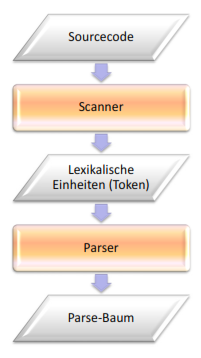
\includegraphics[width=0.6\textwidth]{pics/Lexikalische_Analyse.png}
 		\end{minipage}
 		
 	\subsection{Lexikalische Einheiten (Token) \verweis{4.2}}
 		\subsubsection{Gross- und Kleinschreibung}
 			\begin{compactitem}
 				\item C unterscheidet Gross- und Kleinschreibung, d.h. C ist case-sensitive
 				\item Die reservierten Wörter sind immer klein geschrieben
 				\item $alpha$ und $Alpha$ sind unterschiedliche Namen
 				\item Solche Feinheiten, bei denen sich zwei Namen nur in der Gross- bzw. Kleinschreibung einzelner Buchstaben unterscheiden, sollen unbedingt vermieden werden (fehleranfällig)
 			\end{compactitem}
 		\subsubsection{Kommentare}
 			\begin{compactitem}
 				\item Kommentare sollen die Verständlichkeit des Programms erhöhen
 				\item Sie werden vom Preprocessor (allererster Compile-Schritt) entfernt. Sie sind im
 				ausführbaren Code nicht mehr enthalten.
 				\item Ein Kommentar muss mit
 				$/*$ und $*/$ eingefasst werden
 				\item Kommentare können auch über mehrere Zeilen reichen, sie dürfen aber nicht
 				verschachtelt werden
 				\item Zeilenkommentare beginnen mit einem Doppelslash
 				$//$. Sie reichen ab dem
 				Doppelslash bis zum Ende der Zeile
 			\end{compactitem}
 		\subsubsection{Namen \verweis{4.2.1}}
 			\begin{minipage}[t]{5 cm}
 				Namen bezeichnen in C:
 				\begin{compactitem}
					\item Variablen
					\item Funktionen
					\item Tags von Strukturen, \\Unions, Bitfeldern, \\Enumerations
					\item Komponenten von Strukturen
					\item Enum Konstanten
					\item Typnamen (typedef)
					\item Marken (Label)
					\item Makronamen ($\#define$)
 				\end{compactitem}
 			\end{minipage}
 			\hspace*{1.0cm}
 			\begin{minipage}[t]{5 cm}
	 			Namen können bestehen aus:
	 			\begin{compactitem}
					\item Buchstaben a-z, A-Z
					\item Ziffern 0-9
					\item Underscore \_
	 			\end{compactitem}
	 			\vspace*{0.2cm} 
	 			Das erste Zeichen eines Namens darf keine Ziffer sein!
	 		\end{minipage}
	 		\hspace*{1.0cm}
	 		\begin{minipage}[t]{6 cm}
		 		Styleguide Variablen \& Funktionen:
		 		\begin{compactitem}
		 			\item mit Kleinbuchstaben beginnen	 			
		 			\item erster Buchstaben von zusammengesetzten Wörtern ist gross	
		 			\item keine Underscores
		 		\end{compactitem}
		 		\vspace*{0.2cm} 
		 		Beispiele: $counter$, $maxSpeed$, \\$getCount()$, $init()$, $setMaxSpeed()$	
	 		\end{minipage}	
		
 		\subsubsection{Reservierte Wörter \verweis{4.2.2}}
 			In ANSI C sind 32 reservierte Schlüsselwörter definiert. Sie sind stets klein geschrieben und dürfen nicht als Namen (z.B. für Variablen) verwendet werden.\\\\
 			\begin{minipage}[c]{2.2 cm}
	 			\begin{compactitem}
	 				\item $auto$
	 				\item $break$				
	 				\item $case$				
	 				\item $char$ 								
	 			\end{compactitem}
 			\end{minipage}
 			\begin{minipage}[c]{2.3 cm}
	 			\begin{compactitem}	
	 				\item $const$
	 				\item $continue$			
	 				\item $default$
	 				\item $do$	 	
	 			\end{compactitem}
 			\end{minipage}
 			\begin{minipage}[c]{2.2 cm}
	 			\begin{compactitem}	
	 			 	\item $double$
	  			 	\item $else$	
	 			 	\item $enum$ 			 	
	 			 	\item $extern$ 		 		 	
	 			\end{compactitem}
 			\end{minipage}
 			\begin{minipage}[c]{2.2 cm}
	 			\begin{compactitem}	
	 			 	\item $float$			 	
	 			 	\item $for$			 	
	 			 	\item $goto$		
	 			 	\item $if$			 	
	 			\end{compactitem}
	 		\end{minipage}
 			\begin{minipage}[c]{2.2 cm}
	 			\begin{compactitem} 
	 			 	\item $int$			 	
	 			 	\item $long$ 		 	
	 			 	\item $register$			 	
	 			 	\item $return$ 			 	
	 			\end{compactitem}
	 		\end{minipage}
 			\begin{minipage}[c]{2.2 cm}
	 			\begin{compactitem}		 
	 			 	\item $short$ 			 	
	 			 	\item $signed$ 			 	
	 			 	\item $sizeof$ 			 	
	 			 	\item $static$	
	 			\end{compactitem}
	 		\end{minipage}
 			\begin{minipage}[c]{2.2 cm}
	 			\begin{compactitem}		 	
	 			 	\item $struct$ 		 	
	 			 	\item $switch$ 			 	
	 			 	\item $typedef$ 			 	
	 			 	\item $union$ 			 	
	 			\end{compactitem}
	 		\end{minipage}
 			\begin{minipage}[c]{2.4 cm}
	 			\begin{compactitem}		 	
	 			 	\item $unsigned$ 			 	
	 			 	\item $void$	
	 			 	\item $volatile$		 	
	 			 	\item $while$
	 			\end{compactitem}
	 		\end{minipage}
	 		
	 		\begin{minipage}[t]{8 cm}
		 		\subsubsection{Symbolische Konstanten \verweis{4.2.3}}
		 			Haben Namen, der ihren Wert repräsentiert.
		 			\begin{compactitem}
		 				\item Können mit dem Präprozessor-Befehl $\#define$ eingeführt werden:\\
		 				$\#define$ $PI$ \ \ $3.1415$\\
		 				$\#define$ $LIST\_LENGTH$ \ \ $40$
		 				\item Verhindern von "Magic numbers"
		 				\item Vereinfacht Änderungen
		 				\item Styleguide: Symbolische $\#define$-Konstanten werden aus Grossbuchstaben und Underscores gebildet (keine Kleinbuchstaben) 			 	
		 			\end{compactitem}
		 	\end{minipage}
		 	\hspace*{1.0 cm}
		 	\begin{minipage}[t]{9 cm}
 				\subsubsection{Literale Konstanten \verweis{4.2.3}}
 					Haben keinen Namen. Werden durch ihren Wert repräsentiert.
 					\begin{compactitem}
	 					\item Ganzzahlige Konstanten (default: int):\\
	 					$254$ $(dez)$, $035$ $(okt)$, $0x3f$ $(hex)$, $-34$, $14L$ $(long)$,\\ $14U$ $(unsigned)$, $14UL$ $(unsigned long)$
	 					\item Zeichenkonstanten:\\
	 					$'c'$, $'\textbackslash n'$, $'\textbackslash x4a'$ $(ASCII$ $hex)$, $'\textbackslash014'$ $(ASCII$ $okt)$, \\$'\textbackslash \textbackslash'$, $L'a'$ $(Double Byte)$
	 					\item Gleitpunktkonstanten (default: double):\\
	 					$254.89$, $-13.0$, $3.45e23$ $(exp. Schreibweise)$, \\ $4.65f$ $(float-Konstante)$,  $3.14159L$ $(long$ $double)$
	 					\item Aufzählungskonstanten		 				 			 	
 					\end{compactitem}
 			\end{minipage}
 		\subsubsection{Konstante Zeichenkette (String) \verweis{4.2.4}}
 			\begin{minipage}[t]{9 cm}
 				\begin{compactitem}
 					\item begrenzt mit $"'  "'$
 					\item (automatisch) abgeschlossen mit Nullzeichen $'\textbackslash0'$
 				\end{compactitem}	
 			\end{minipage}
 			\hspace*{0.5cm}
 			\begin{minipage}[t]{9 cm}
 				Beispiel $"'Ritchie"'$\\
 				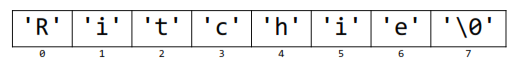
\includegraphics[width=0.6\textwidth]{pics/Zeichenkonstante.png}
 			\end{minipage}
 	\subsection{Enumerations (Aufzählungstyp)}
 		\begin{minipage}[t]{9 cm}
	 		\vspace*{-0.5cm}
	 		\lstinputlisting[language=C,tabsize=2]{code/enum1.c}
 		\end{minipage}
 		\hspace*{0.5 cm}
 		\begin{minipage}[t]{8 cm}
 			\begin{compactitem}
 				\item Aufzählungskonstanten haben einen konstanten ganzzahligen Wert.
 				\item Die erste Konstante erhält den Wert $0$, die zweite $1$, etc.
 				\item Werte können auch explizit zugewiesen werden
 			\end{compactitem}
 		\end{minipage}
 		
 		\subsubsection{Anonyme Enumerations}
 			$enums$ können auch verwendet werden, um ganzzahlige symbolische Konstanten zu definieren. Der $enum$ erhält dann keinen Namen, er wird nur dazu verwendet, die einzelnen Konstanten festzulegen. Bessere Alternative zu $\#define$ für ganzzahlige Konstanten!!
 			\lstinputlisting[language=C,tabsize=2]{code/enum2.c}
 			\vspace*{0.5cm}